\documentclass[titlepage]{article}

\usepackage{color}
\usepackage{tikz}
\usepackage{hyperref}
\usepackage{array}

\usetikzlibrary{shapes,arrows}

\tikzset{%
    block/.style = {draw, thick, rectangle, align=left, node distance=3cm},
}

\hypersetup{
    urlcolor=cyan
}

\title{Complete Quadcopter Design and Implementation}
\date{\today}
\author{Nathan Lilienthal}

\begin{document}

\maketitle

\tableofcontents
\clearpage

\section{Hardware Specification}

This section outlines the main components for the design of the control board.
Smaller parts like resistors or oscillators are omitted. This document is
concerned with the functional capabilities of the design, not the electrical
implementation. For more details on the electrical implementation of this design
please reference the schematic.

\subsection{Part List}

The part list is of the following form:

\begin{description}
  \item[Long Name ($Short Name$)]\hfill\\
  Description
\end{description}

In general the short names of parts will be used for brevity. Long names specify
the actual part, short names specify the functionality.

\begin{description}
  \item[Atmel ATSAM4SD32CA ($\mu C$)]\hfill\\
  This Atmel ARM Cortex-M4 Processor, serving as the main processing unit for the
  quadcopter.
  \item[InvenSense MPU-9250 ($IMU$)]\hfill\\
  The second item
  \item[Bosch Sensortec BMP-183 ($BMP$)]\hfill\\
  The third etc
  \item[SkyTraq Venus638FLPx ($GPS$)]\hfill\\
  The third etc
  \item[XBee Pro 900 RPSMA ($RF$)]\hfill\\
  The third etc
  \item[Turnigy Plush 25A Electronic Speed Controller ($ESC$)]\hfill\\
  The third etc
\end{description}

% \begin{itemize}
%     \item Atmel ATSAM4SD32CA
%     \url{http://www.digikey.com/product-detail/en/ATSAM4SD32CA-AU/ATSAM4SD32CA-AU-ND/4010086}
%     \item BMP183 (\$4.80)\\
%     \url{http://www.digikey.com/product-detail/en/BMP183/828-1034-1-ND/3884363}
%     \item MPU-9250 (\$12.82)\\
%     \url{http://www.digikey.com/product-detail/en/MPU-9250/1428-1019-1-ND/4626450}
%     \item Venus638FLPx (\$49.95)\\
%     \url{https://www.sparkfun.com/products/11058}
%     \item XBee Pro 900 RPSMA (\$54.95)\\
%     \url{https://www.sparkfun.com/products/9099}
%     \item Turnigy Plush 25A ESC (\$13.45)\\
%     \url{http://www.hobbyking.com/hobbyking/store/__2163__TURNIGY_Plush_25amp_Speed_Controller.html?gclid=CPfrm-fm0cQCFViUfgod_hgA0g}
% \end{itemize}

\subsection{Block Diagram}

\begin{figure}[h]
    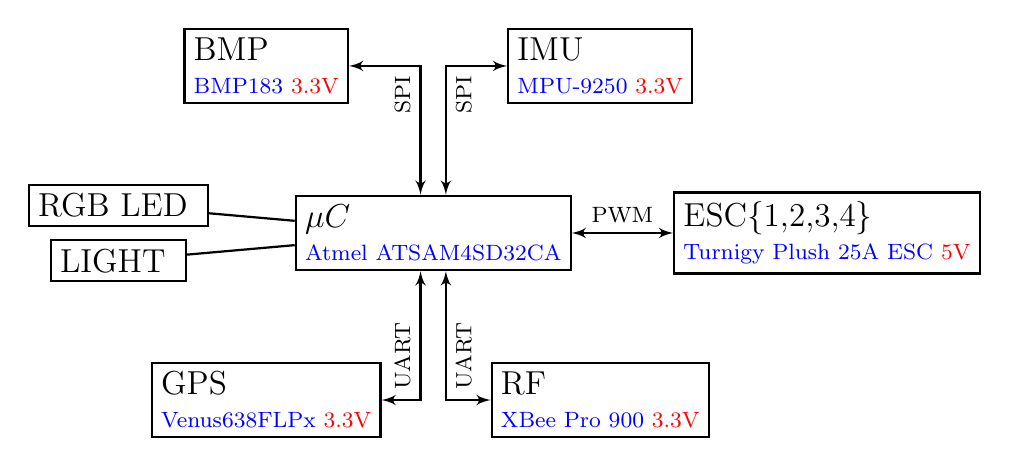
\begin{tikzpicture}[auto, thick, node distance=2cm,>=latex']
        \draw
            node at (0,0) [block] (mcu)
            {
                \large{$\mu C$}\\
                \textcolor{blue}{\footnotesize{Atmel ATSAM4SD32CA}}
            }
            node [block, above right of=mcu] (imu)
            {
                \large{IMU}\\
                \footnotesize{\textcolor{blue}{MPU-9250} \textcolor{red}{3.3V}}
            }
            node [block, above left of=mcu] (bmp)
            {
                \large{BMP}\\
                \footnotesize{\textcolor{blue}{BMP183} \textcolor{red}{3.3V}}
            }
            node [block, below right of=mcu] (rf)
            {
                \large{RF}\\
                \footnotesize{\textcolor{blue}{XBee Pro 900} \textcolor{red}{3.3V}}
            }
            node [block, below left of=mcu] (gps)
            {
                \large{GPS}\\
                \footnotesize{\textcolor{blue}{Venus638FLPx} \textcolor{red}{3.3V}}
            }
            node [block, right of=mcu, node distance=5cm] (escs)
            {
                \large{ESC\{1,2,3,4\}}\\
                \footnotesize{\textcolor{blue}{Turnigy Plush 25A ESC} \textcolor{red}{5V}}
            }
            node [block, left of=mcu, yshift=1em, node distance=4cm] (rgb_led)
            {
                \large{RGB LED}
            }
            node [block, left of=mcu, yshift=-1em, node distance=4cm] (light)
            {
                \large{LIGHT}
            };

        \draw[<->]([xshift=2em]mcu) |- node[sloped, below left, rotate=90]
            {\footnotesize{SPI}} (imu);
        \draw[<->]([xshift=-2em]mcu) |- node[sloped, above left, rotate=90]
            {\footnotesize{SPI}} (bmp);
        \draw[<->]([xshift=2em]mcu) |- node[sloped, below right, rotate=90]
            {\footnotesize{UART}} (rf);
        \draw[<->]([xshift=-2em]mcu) |- node[sloped, above right, rotate=90]
            {\footnotesize{UART}} (gps);
        \draw[<->](mcu) -- node
            {\footnotesize{PWM}} (escs);
        \draw[-](mcu) -- node {} (rgb_led);
        \draw[-](mcu) -- node {} (light);
    \end{tikzpicture}

    \caption{Functional Block Diagram}
\end{figure}

\subsection{Part Descriptions}

Aside from the datasheets, which should cover everything needed, this section
outlines the most important information for each part. Some of the details in
this section were discovered through testing.

\subsubsection{Turnigy Plush 25A ESC}

This part has no reliable electronic datasheet. The documentation is basically
a manual. Some details about Voltage and Current are specified, but timings
and operations are completely missing.

% \begin{tabular}{|l|l|l|}
% \cline{2-3}
% & Value & Unit\\
% \cline{1-3}
% PWM Period & 50 & Hz\\
% \hline
% 11&22&33\\
% \hline
% 1.1&2.2&3.3\\
% \hline
% \end{tabular}

\end{document}